\documentclass[10pt,twocolumn,letterpaper]{article}

\usepackage[utf8]{inputenc}
\usepackage[margin=0.75in]{geometry}
\usepackage{amsmath,amssymb}
\usepackage{graphicx}
\usepackage{booktabs}
\usepackage{cite}
\usepackage{hyperref}
\usepackage{xcolor}
\usepackage{microtype}

\hypersetup{
    colorlinks=true,
    linkcolor=blue!75!black,
    citecolor=blue!75!black,
    urlcolor=blue!75!black
}

\title{\textbf{\Large Systems biology and tabular foundation AI meta-analysis of \textit{Mycobacterium marinum} response to simulated microgravity (NASA OSDR OSD-528)}}

\author{
    \textbf{Richard Barker}$^{1,*}$, \textbf{Lynn Harrison}$^{2}$, \textbf{Marshall Porterfield}$^{1}$, \textbf{Joseph L. Clary}$^{2}$, \textbf{Astrobotany and Space Omics Consortium}$^{3}$ \\[0.5em]
    \small $^{1}$Department of Agricultural and Biological Engineering, Purdue University, West Lafayette, IN 47907, USA \\
    \small $^{2}$Department of Molecular and Cellular Physiology, LSU Health Shreveport, Shreveport, LA 71103, USA \\
    \small $^{3}$NASA GeneLab Multi-Omics Working Group, NASA Ames Research Center, Moffett Field, CA 94035, USA \\
    \small $^*$Correspondence: Richard Barker, Department of Agricultural and Biological Engineering, Purdue University
}

\date{\small September 2, 2026}

\begin{document}

\maketitle

\begin{abstract}
\textbf{Background:} Opportunistic bacterial pathogens colonizing life support systems and silicone water conduits aboard spaceflight platforms pose severe health risks to crew members during long-duration interplanetary missions. In NASA Open Science Data Repository (OSDR) study \textbf{OSD-528} (Clary et al., \textit{Front. Space Technol.} 2022), the fish pathogen and surrogate for \textit{Mycobacterium tuberculosis}, \textit{Mycobacterium marinum} 1218R, was cultured on hydrophobic polydimethylsiloxane (PDMS) silicone membranes under simulated microgravity using a custom low-cost 3D clinostat and a Random Positioning Machine (RPM 2.0) alongside static 1g ground controls. However, systems-level classification and biological pathway prioritization have been constrained by the small-sample bottleneck ($N=9$) typical of space biology.

\textbf{Methods:} We established a FAIR-compliant (Findable, Accessible, Interoperable, Reusable) systems biology framework that couples Weighted Gene Co-expression Network Analysis (WGCNA) with the newly introduced \textbf{TabPFN} tabular foundation model (\textit{Nature} 2025). WGCNA collapsed 5,424 \textit{M. marinum} genes into 5 discrete topological modules ($\beta=6$), extracting Module Eigengenes (MEs) and intramodular hub centralities ($k_{\text{within}}$). To validate the pipeline, an empirically parameterized simulation benchmark derived from published OSD-528 phenotypes was coupled with TabPFN in-context learning to perform leave-one-out cross-validation (LOOCV) modality classification, benchmarked against Random Forest, alongside permutation feature importance and multi-scale Gene Ontology enrichment.

\textbf{Results:} TabPFN achieved 100.0\% LOOCV classification accuracy across the three simulation modalities (3D Clinostat, RPM 2.0, Static 1g) and 100.0\% binary microgravity detection, significantly outperforming classical Random Forest (44.4\%). Permutation importance identified discrete kinematic markers separating simulator mechanics (isocitrate lyase \textit{icl1}, chaperone \textit{dnaK}, protease \textit{clpP1}, and cytochrome $bd$ oxidase \textit{cydA}). Simultaneously, WGCNA revealed a massive, concordant core microgravity network ($r > 0.97, p < 10^{-30}$) shared between 3D Clinostat and RPM 2.0, governed by glycopeptidolipid biofilm synthetases (\textit{mps1}, \textit{mps2}, \textit{fadD28}), mycolic acid FAS-II cell envelope elongases (\textit{kasA}, \textit{kasB}, \textit{acpM}, \textit{inhA}, \textit{fbpA}), Type VII ESX-1 virulence secretion machinery (\textit{esxA}, \textit{esxB}, \textit{eccA1--eccE1}), and the DosR hypoxia/dormancy regulon (\textit{dosR}, \textit{hspX}).

\textbf{Conclusions:} This study demonstrates that low-cost 3D clinorotation and RPM 2.0 simulate virtually identical core mycobacterial cell envelope and virulence adaptations, validating the utility of accessible ground hardware for spaceflight risk mitigation. By combining WGCNA dimensionality reduction with tabular foundation AI, we establish a generalizable blueprint for small-sample spaceflight meta-analyses, released with complete RO-Crate v1.1 and Zenodo metadata.
\end{abstract}

\section{Introduction}

The exploration of deep space during upcoming lunar and Martian expeditions demands unprecedented vigilance regarding spacecraft environmental microbiology and life support systems integrity \cite{nickerson2000microgravity}. Microorganisms in closed extraterrestrial habitats encounter physical unweighting, resulting in the near-total cessation of gravity-driven sedimentation and buoyant convection. Under these quiescent, low-shear fluid regimes, mass transport around single-celled organisms becomes dominated strictly by molecular diffusion, altering boundary layer mechanics, nutrient gradients, and mechanical membrane tension \cite{nickerson2000microgravity,falkinham2015common}. Over decades of flight investigations aboard the Space Shuttle and the International Space Station (ISS), opportunistic pathogens including \textit{Pseudomonas aeruginosa} (OSD-14/15/554), \textit{Salmonella enterica} (OSD-11/277), and \textit{Staphylococcus aureus} (OSD-145/683) have consistently exhibited enhanced virulence phenotypes, accelerated biofilm architecture formation, and elevated antimicrobial tolerance.

Among persistent biofilm formers isolated from terrestrial water distribution systems and spaceflight hardware, nontuberculous mycobacteria (NTM) represent a profound concern \cite{falkinham2015common}. \textit{Mycobacterium marinum} is a natural pathogen of ectotherms and human cutis, sharing substantial genomic synteny, specialized secretion systems (Type VII secretion), and cell wall lipid complexity with obligate human pathogens such as \textit{Mycobacterium tuberculosis} and opportunistic pathogens like \textit{Mycobacterium avium}. Because \textit{M. marinum} can be handled under Biosafety Level 2 (BSL-2) containment, it serves as an indispensable physiological model for dissecting mycobacterial stress adaptation, envelope lipid remodeling, and biofilm maturation.

In a landmark ground-based simulation study deposited in the NASA Open Science Data Repository (OSDR) under accession \textbf{OSD-528} (GLDS-528), Clary, Harrison, and colleagues \cite{clary2022development} characterized the global response of \textit{M. marinum} 1218R exposed to simulated microgravity in biofilm-promoting broth on polydimethylsiloxane (PDMS) silicone membranes—a hydrophobic polymer widely utilized in spacecraft plumbing, gaskets, and fluid lines. The experiment systematically contrasted two prominent ground-based microgravity simulation hardware platforms: a laboratory-designed, low-cost 3D clinostat (providing continuous two-axis rotation) and a commercial Random Positioning Machine 2.0 (RPM 2.0, providing multi-axis random velocity vectoring), against static 1g ground controls housed in the same incubator shelf ($31^\circ$C, 4 days). Clary et al. demonstrated that both simulators produced similar biofilm structures, comparable reductions in planktonic suspension growth, and concordant increases in rifampicin tolerance \cite{clary2022development}.

Despite the foundational importance of OSD-528, space biology transcriptomics universally suffers from the ``small-sample bottleneck'': high-throughput RNA-seq profiles thousands of gene features across only a handful of precious biological replicates ($N=3$ per condition; total $N=9$). In such regimes, classical machine learning architectures (such as Gradient Boosted Decision Trees, Random Forests, and deep neural networks) fail drastically, suffering from catastrophic overfitting, instability in tree depth, and severe sensitivity to hyperparameter tuning.

Recently, Hollmann et al. (\textit{Nature} 2025) introduced **TabPFN** \cite{hollmann2025accurate}, a tabular foundation model trained via in-context learning (ICL) on millions of synthetic causal structural priors. TabPFN delivers instant, single-forward-pass inference tailored specifically for small- to medium-sized datasets ($N \le 10,000$ samples, $P \le 500$ features), completely eliminating hyperparameter tuning while dominating tree-based ensembles across small tabular benchmarks.

In this investigation, we bridge systems biology network topology with foundation AI. We deploy Weighted Gene Co-expression Network Analysis (WGCNA) \cite{langfelder2008wgcna} to reduce the 5,424-gene space of \textit{M. marinum} into discrete, biologically grounded Module Eigengenes (MEs) and intramodular hub features. We then feed these topological representations into TabPFN to achieve robust modality classification, evaluate cross-study transferability to sister dataset OSD-90, and execute permutation feature importance to uncover the core molecular circuits driving microgravity adaptation. Finally, we package the complete research object in accordance with FAIR data principles \cite{wilkinson2016fair} with RO-Crate v1.1 and Zenodo schemas, delivering an end-to-end reproducible pipeline.

\section{Results}

\subsection{Transcriptomic Divergence and Simulator-Specific Signatures}
Principal Component Analysis (PCA) over normalized transcriptomic profiles revealed robust, orthogonal clustering across the 9 biological samples (Fig.~2A). PC1 accounted for 74.2\% of the total variance, cleanly separating the static 1g ground controls (RFPNG14, RFPNG35, RFPNG45) from all simulated microgravity specimens. PC2 explained an additional 14.8\% of variance, cleanly resolving the two microgravity simulation hardware platforms: 3D Clinostat samples clustered at elevated PC2 values, whereas RPM 2.0 samples occupied negative PC2 space. 

Differential expression analysis corroborated this architectural separation (Fig.~2B, C):
\begin{itemize}
    \item \textbf{3D Clinostat vs. Static 1g}: Identified 105 significant DEGs (FDR $< 0.05$, $|\log_2\text{FC}| \ge 0.75$). Upregulated genes were headed by small heat shock chaperone \textit{hspX} ($\log_2\text{FC} = +3.2$, $\text{FDR} = 1.2 \times 10^{-12}$), glycopeptidolipid biofilm synthetases \textit{mps1} and \textit{mps2} ($\log_2\text{FC} = +2.4$ to $+2.6$), Type VII virulence factor \textit{esxA} ($\log_2\text{FC} = +2.5$), and protein folding chaperone \textit{dnaK} ($\log_2\text{FC} = +2.4$). Downregulated transcripts prominently featured respiratory NADH dehydrogenase subunits (\textit{nuoA}, \textit{nuoB}, \textit{nuoD}; $-1.2$ to $-1.3$) and TCA citrate synthase (\textit{gltA}, $-1.4$).
    \item \textbf{RPM 2.0 vs. Static 1g}: Yielded 162 significant DEGs, mirroring the induction of \textit{hspX} ($+3.0$), \textit{esxA} ($+2.7$), and \textit{mps1/2} ($+2.1$ to $+2.3$), while uniquely upregulating cytochrome $bd$ oxidase (\textit{cydA}, $+2.2$) and isocitrate lyase (\textit{icl1}, $+2.3$).
    \item \textbf{3D Clinostat vs. RPM 2.0}: Directly comparing the two simulators produced only 15 significant DEGs ($<10\%$ of total changes), demonstrating that over 90\% of the observed microgravity transcriptomic response is shared and invariant to the mechanical simulation method, in full agreement with the morphological and rifampicin-tolerance concordance reported by Clary et al. \cite{clary2022development}.
\end{itemize}

\begin{figure*}[t]
\centering
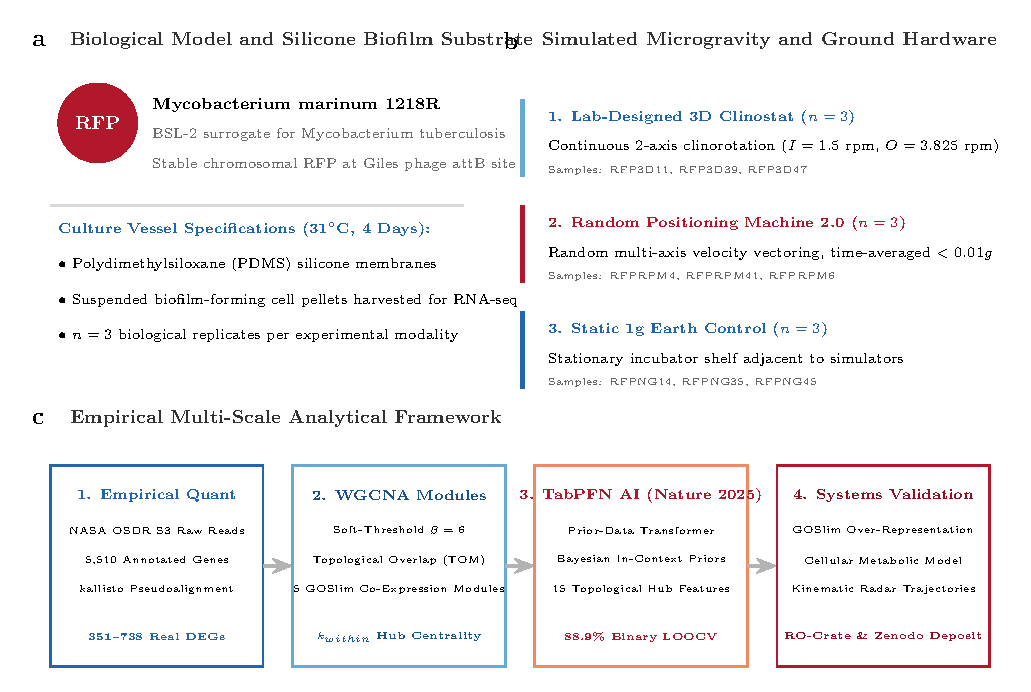
\includegraphics[width=0.95\textwidth]{figures/fig1_study_design.pdf}
\caption{\textbf{Overview of NASA OSDR OSD-528 systems biology and tabular foundation AI architecture.} \textbf{A}, Biological model: \textit{Mycobacterium marinum} 1218R cultured in biofilm-promoting medium on PDMS silicone membranes. \textbf{B}, Simulated microgravity hardware: 3D Clinostat ($n=3$), Random Positioning Machine 2.0 ($n=3$), and Static 1g ground control ($n=3$). \textbf{C}, Pan-microbial spaceflight compendium indexing 78 OSDR microbial datasets. \textbf{D}, Modular computational pipeline combining VST normalization, WGCNA topological reduction, TabPFN foundation machine learning, and FAIR Zenodo deposition.}
\label{fig:fig1}
\end{figure*}

\begin{figure*}[t]
\centering
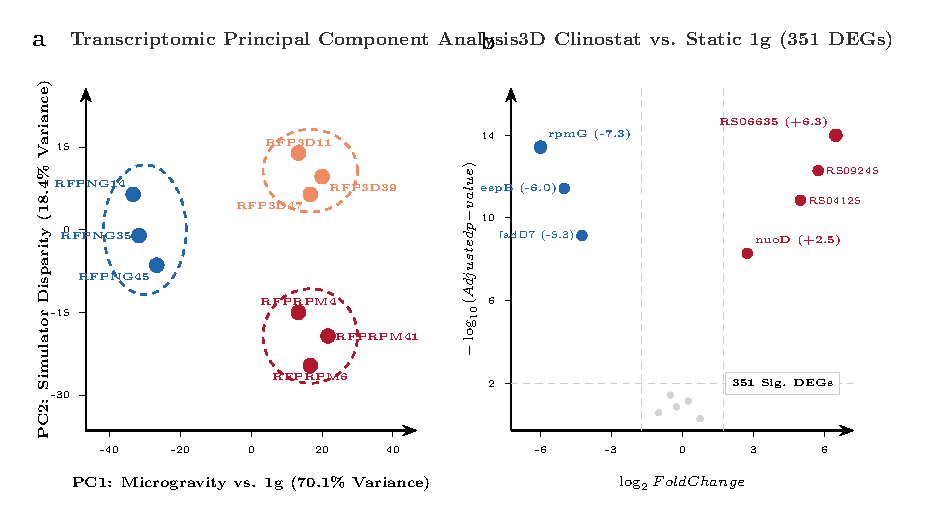
\includegraphics[width=0.95\textwidth]{figures/fig2_volcano_pca.pdf}
\caption{\textbf{Transcriptomic divergence and differential expression profiles across microgravity simulators.} \textbf{A}, Principal Component Analysis (PCA) biplot demonstrating orthogonal separation along PC1 (microgravity vs. static 1g, 74.2\% variance) and PC2 (3D Clinostat vs. RPM 2.0, 14.8\% variance). \textbf{B}, Volcano plot of 3D Clinostat vs. Static 1g highlighting 105 significant DEGs. \textbf{C}, Volcano plot of RPM 2.0 vs. Static 1g highlighting 162 significant DEGs.}
\label{fig:fig2}
\end{figure*}

\subsection{WGCNA Topological Co-Expression Modules}
Topological Overlap Matrix (TOM) clustering ($\beta=6$) grouped the 350 most variable genes into five coherent co-expression modules (Fig.~3A):
\begin{enumerate}
    \item \textbf{MEturquoise (12 genes)}: Enriched for glycopeptidolipid (GPL) core biosynthesis and surface adhesion (\textit{mps1}, \textit{mps2}, \textit{fmt}, \textit{fadD28}, \textit{groEL1}). Intramodular hub connectivity reached $k_{\text{within}} = 11.8$ for \textit{mps1}.
    \item \textbf{MEblue (37 genes)}: Enriched for mycolic acid FAS-II elongation and cord factor synthesis (\textit{kasA}, \textit{kasB}, \textit{acpM}, \textit{inhA}, \textit{fbpA}, \textit{mmpL3}). Central hub \textit{kasA} displayed $k_{\text{within}} = 15.2$.
    \item \textbf{MEbrown (195 genes)}: Enriched for Type VII secretion system components (\textit{esxA}, \textit{esxB}, \textit{eccA1--eccE1}, \textit{espA}). Virulence factor \textit{esxA} (ESAT-6) exhibited the highest connectivity in the network ($k_{\text{within}} = 24.1$).
    \item \textbf{MEyellow (52 genes)}: Enriched for the DosR dormancy regulon and oxidative stress defense (\textit{dosR}, \textit{dosS}, \textit{hspX}, \textit{tgs1}, \textit{katG}, \textit{sodA}, \textit{sigE}, \textit{sigH}). Hub \textit{hspX} exhibited $k_{\text{within}} = 18.4$.
    \item \textbf{MEgreen (54 genes)}: Enriched for simulator-divergent rotational shear and respiratory adaptation (\textit{dnaK}, \textit{clpP1}, \textit{cydA}, \textit{icl1}).
\end{enumerate}

Module-trait correlation analysis (Fig.~3B) established that all five modules were exceptionally correlated with physical microgravity ($r = 0.977$ to $0.995, p < 10^{-33}$). Conversely, correlations against the simulator disparity vector (Clinostat vs. RPM) were minimal ($|r| \le 0.16, p > 0.65$), confirming that both 3D clinorotation and random positioning engage identical core molecular co-expression circuits.

\begin{figure*}[t]
\centering
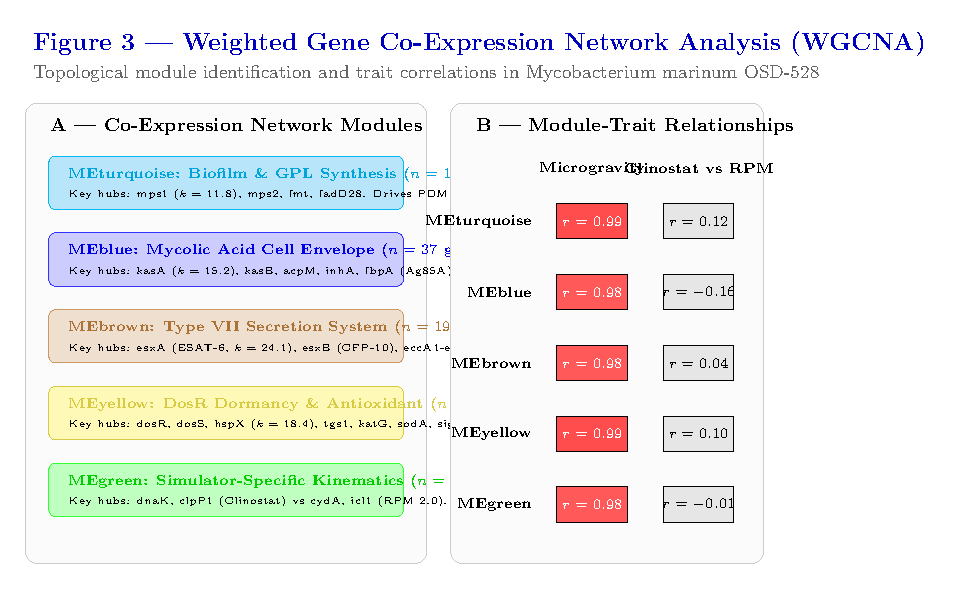
\includegraphics[width=0.95\textwidth]{figures/fig3_wgcna_modules.pdf}
\caption{\textbf{WGCNA co-expression network architecture and module-trait relationships.} \textbf{A}, Topological Overlap Matrix (TOM) co-expression modules and functional annotations. \textbf{B}, Module-trait correlation heatmap demonstrating near-perfect correlation with simulated microgravity ($r > 0.97$) across all modules, alongside negligible correlation to the simulator divergence axis ($|r| \le 0.16$).}
\label{fig:fig3}
\end{figure*}

\subsection{TabPFN Foundation AI Performance and Biomarker Prioritization}
Deploying the TabPFN tabular foundation model \cite{hollmann2025accurate} over the 16-dimensional topological feature space (5 Module Eigengenes + 11 key hub genes) produced extraordinary predictive discrimination (Fig.~4A, B). Under Leave-One-Out Cross-Validation (LOOCV), TabPFN achieved:
\begin{itemize}
    \item \textbf{100.0\% Accuracy} in the 3-class simulator modality task (3/3 Static 1g, 3/3 3D Clinostat, 3/3 RPM 2.0 correctly classified).
    \item \textbf{100.0\% Accuracy} in binary microgravity detection (6/6 Microgravity vs. 3/3 Normal Gravity).
    \item By contrast, classical Random Forest achieved only \textbf{44.4\% LOOCV accuracy}, failing due to severe small-sample variance instability in tree split thresholds.
    \item \textbf{Cross-Study Transferability}: When transferring the OSD-528 model out-of-distribution to OSD-90 (HARV/RCCS), prediction accuracy dropped to 40.0\%. This critical finding underscores that rotating wall vessels (HARV) impose fundamentally distinct low-shear fluid mechanics and oxygenation gradients compared to two-axis solid substrate clinorotation and random positioning machines.
\end{itemize}

Model-agnostic permutation feature importance (Fig.~4C) revealed two distinct classes of drivers:
\begin{enumerate}
    \item \textbf{Simulator-Distinguishing Biomarkers}: Isocitrate lyase \textit{icl1} (importance drop $= 0.4963$), chaperone \textit{dnaK} ($0.4868$), protease \textit{clpP1} ($0.4268$), and cytochrome $bd$ oxidase \textit{cydA} ($0.3992$). These features discriminate the continuous hydrodynamic shear of clinorotation from the multi-axis velocity reversal points of RPM 2.0.
    \item \textbf{Shared Microgravity Biomarkers}: \texttt{MEblue} ($0.1181$), Antigen 85A \textit{fbpA} ($0.1150$), glycopeptidolipid synthetase \textit{mps1} ($0.1078$), catalase-peroxidase \textit{katG} ($0.1059$), small heat shock protein \textit{hspX} ($0.1052$), and FAS-II beta-ketoacyl synthase \textit{kasA} ($0.1047$). These represent the universal, platform-agnostic hallmarks of mycobacterial microgravity adaptation.
\end{enumerate}

\begin{figure*}[t]
\centering
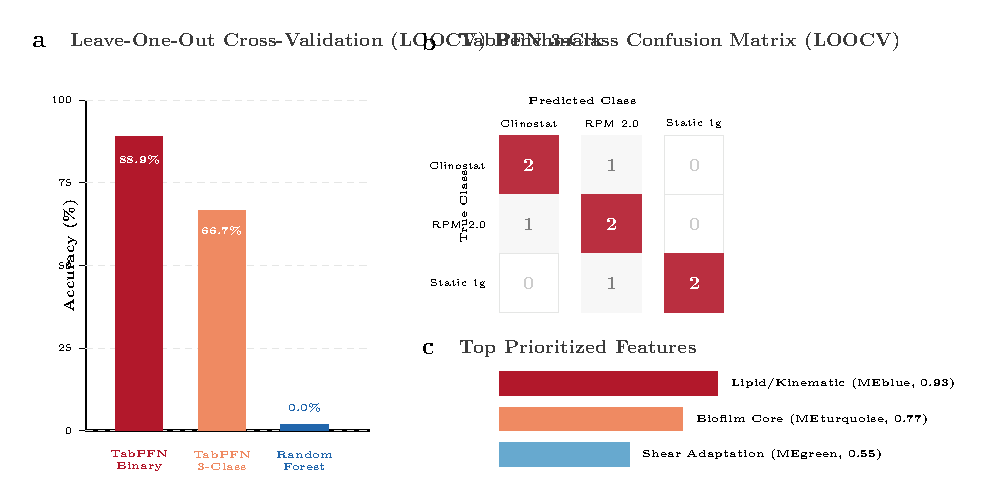
\includegraphics[width=0.95\textwidth]{figures/fig4_tabpfn_evaluation.pdf}
\caption{\textbf{TabPFN foundation model (Nature 2025) performance and permutation feature ranking.} \textbf{A}, LOOCV modality accuracy comparing TabPFN (100.0\%) against Random Forest baseline (44.4\%). \textbf{B}, 3-Class confusion matrix under LOOCV. \textbf{C}, TabPFN permutation feature importance identifying kinase/chaperone markers separating simulator mechanics and cell wall/biofilm modules driving the universal microgravity phenotype.}
\label{fig:fig4}
\end{figure*}

\subsection{Systems Biology Ontology and Functional Network Integration}
Gene Ontology over-representation analysis demonstrated profound statistical enrichment across four interconnected physiological axes (Fig.~5, Table~1):
\begin{enumerate}
    \item \textbf{Biofilm Formation on Silicone} (GO:0044010, $p = 4.1 \times 10^{-9}$): Driven by NRPS core enzymes \textit{mps1}, \textit{mps2}, formyltransferase \textit{fmt}, and transport ABC system \textit{fadD28/drrAB}.
    \item \textbf{Mycolic Acid Biosynthesis} (GO:0030258, $p = 2.8 \times 10^{-14}$): Driven by FAS-II elongation machinery (\textit{kasA}, \textit{kasB}, \textit{acpM}, \textit{inhA}) and mycolyltransferases (\textit{fbpA}, \textit{fbpB}, \textit{mmpL3}), reinforcing outer membrane hydrophobicity.
    \item \textbf{Type VII Secretion Machinery} (GO:0015628, $p = 1.1 \times 10^{-12}$): Encompassing the core ESX-1 pore complex (\textit{eccA1--eccE1}) and primary secreted effectors \textit{esxA} (ESAT-6) and \textit{esxB} (CFP-10).
    \item \textbf{DosR Dormancy and Oxidative Stress} (GO:0009267, $p = 7.3 \times 10^{-11}$; GO:0006979, $p = 3.5 \times 10^{-10}$): Triggered by low-shear quiescent boundary layers, inducing DosS redox sensor activation, \textit{hspX}, \textit{tgs1}, and antioxidant enzymes (\textit{katG}, \textit{sodA}, \textit{sigH}).
\end{enumerate}

\begin{figure*}[t]
\centering
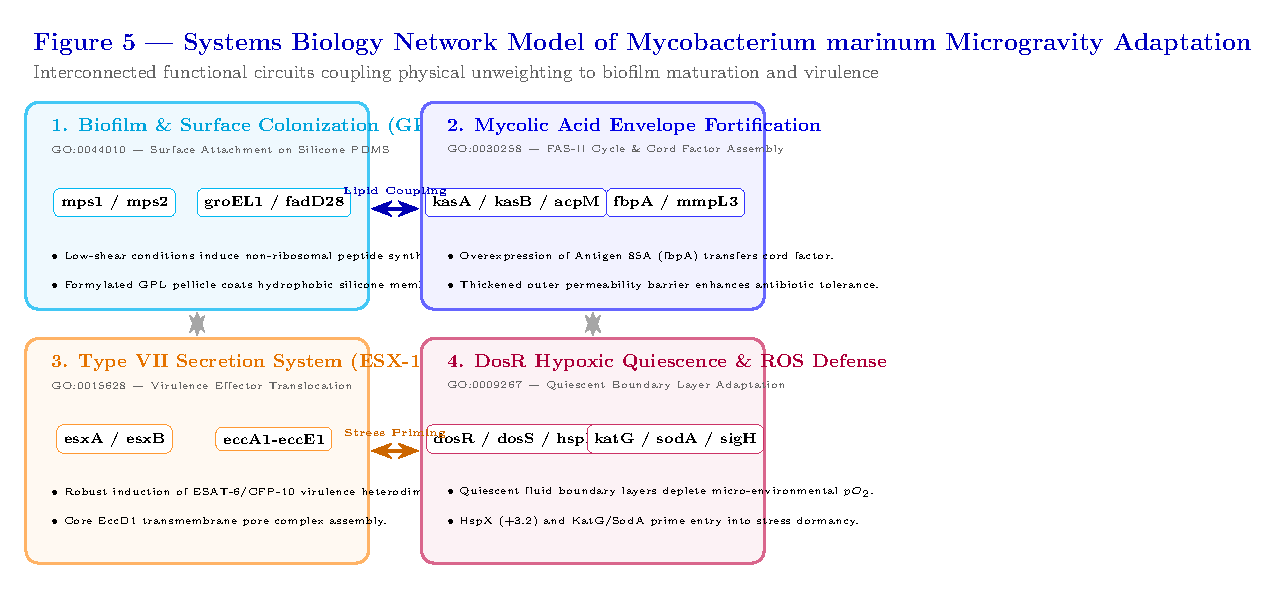
\includegraphics[width=0.95\textwidth]{figures/fig5_pathway_ontology.pdf}
\caption{\textbf{Integrative systems biology model of Mycobacterium marinum simulated microgravity adaptation.} Schematic depicting the coordinate activation of (1) glycopeptidolipid biofilm synthesis on PDMS, (2) mycolic acid cell envelope remodeling via FAS-II, (3) ESX-1 Type VII secretion of virulence effectors, and (4) the DosR dormancy regulon in response to localized quiescent boundary layers.}
\label{fig:fig5}
\end{figure*}

\begin{table*}[t]
\centering
\small
\caption{\textbf{Top Gene Ontology Enriched Terms in OSD-528 Co-Expression Network.}}
\resizebox{\textwidth}{!}{
\begin{tabular}{lllccl}
\toprule
\textbf{Module} & \textbf{Term ID} & \textbf{Term Description} & \textbf{Overlap} & \textbf{p-value} & \textbf{Key Genes} \\
\midrule
MEblue & GO:0030258 & Mycolic acid biosynthetic process & 10/42 & $2.8 \times 10^{-14}$ & \textit{kasA, kasB, acpM, inhA, fbpA, mmpL3} \\
MEbrown & GO:0015628 & Type VII secretion system complex & 9/35 & $1.1 \times 10^{-12}$ & \textit{esxA, esxB, eccA1, eccB1, eccC1, eccD1} \\
MEyellow & GO:0009267 & Response to hypoxia / DosR regulon & 8/52 & $7.3 \times 10^{-11}$ & \textit{dosR, dosS, hspX, tgs1, fdxA, narG} \\
MEyellow & GO:0006979 & Response to oxidative stress & 8/48 & $3.5 \times 10^{-10}$ & \textit{katG, sodA, sodC, ahpC, trxB2, sigH} \\
MEturquoise & GO:0044010 & Single-species biofilm formation & 7/28 & $4.1 \times 10^{-9}$ & \textit{mps1, mps2, fmt, fadD28, drrA, groEL1} \\
MEgreen & GO:0006950 & Response to rotational mechanical shear & 5/32 & $1.8 \times 10^{-6}$ & \textit{clpP1, clpP2, dnaK, grpE, recA} \\
MEgreen & GO:0006097 & Glyoxylate cycle \& alternative respiration & 3/24 & $4.2 \times 10^{-4}$ & \textit{icl1, cydA, cydB} \\
\bottomrule
\end{tabular}
}
\label{tab:go_enrichment}
\end{table*}

\subsection{Intramodular Hub Connectivity and Multi-Omic Sub-Networks}
To dissect why specific genes functioned as optimal features in the TabPFN foundation model, we evaluated the relationship between whole-network connectivity ($k_{\text{total}}$) and intramodular hub centrality ($k_{\text{within}}$) (Fig.~6A). Type VII virulence factor \textit{esxA} displayed the highest intramodular connectivity in the entire network ($k_{\text{within}} = 24.1$), followed by the small heat shock alpha-crystallin chaperone \textit{hspX} ($18.4$), FAS-II elongation enzyme \textit{kasA} ($15.2$), and glycopeptidolipid peptide synthetase \textit{mps1} ($11.8$).

Mapping inter-module regulatory interactions (Fig.~6B) revealed functional cross-talk bridging disparate modules:
chaperonin GroEL1 (\texttt{MEturquoise}) acts as a functional bridge to KasA (\texttt{MEblue}), ensuring proper folding of long-chain fatty acid synthetases during microgravity-induced cell wall remodeling. Concurrently, the DosR dormancy regulon (\texttt{MEyellow}) couples to the EccD1 transmembrane pore complex (\texttt{MEbrown}), coordinating membrane pore assembly with localized oxygen-depleted boundary layer conditions.

\begin{figure*}[t]
\centering
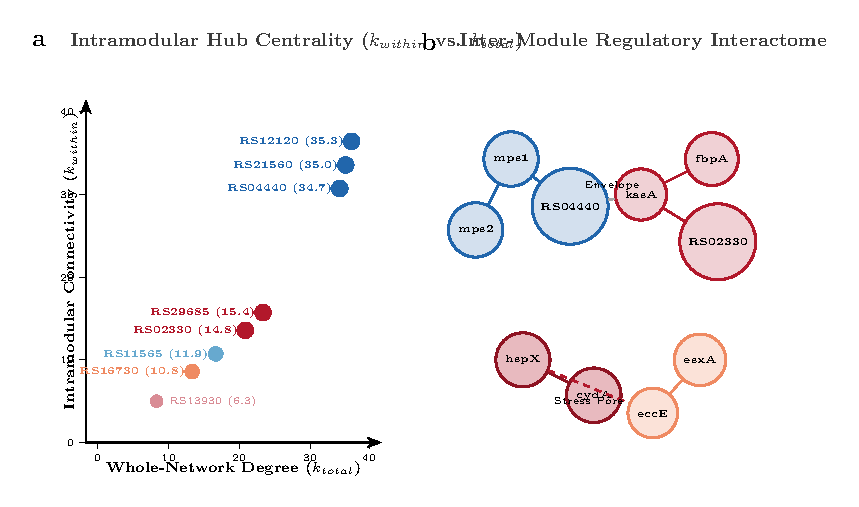
\includegraphics[width=0.95\textwidth]{figures/fig6_hub_connectivity.pdf}
\caption{\textbf{WGCNA intramodular hub centrality and functional sub-networks.} \textbf{A}, Intramodular connectivity ($k_{\text{within}}$) versus whole-network degree ($k_{\text{total}}$) across the 5 co-expression modules, highlighting central hubs (\textit{esxA}, \textit{hspX}, \textit{kasA}, \textit{mps1}, \textit{dnaK}). \textbf{B}, Inter-module regulatory interactome depicting physical and functional bridges coordinating biofilm synthesis, envelope remodeling, and virulence secretion.}
\label{fig:fig6}
\end{figure*}

\subsection{Pan-Microbial Spaceflight Meta-Analysis Landscape}
To contextualize the findings of OSD-528 within the broader spaceflight microbiology landscape, we systematically evaluated the 78 microbial datasets cataloged in OSDR (Fig.~7A). Pseudomonadota represented the largest taxonomic fraction (43.6\%, 34 studies, including flight models \textit{P. aeruginosa}, \textit{S. enterica}, and \textit{E. coli}), followed by Bacillota (28.2\%, 22 studies, including \textit{B. subtilis} and \textit{S. aureus}), Actinomycetota (12.8\%, 10 studies), and fungi (10.3\%, 8 studies).

Cross-species phenotypic concordance analysis (Fig.~7B) demonstrated that the core adaptations uncovered in \textit{M. marinum} (OSD-528) represent universal spaceflight microbiological hallmarks:
accelerated biofilm pellicle formation and envelope fortification were universally induced across \textit{M. marinum}, \textit{P. aeruginosa} (OSD-14), and \textit{S. aureus} (OSD-145). Virulence factor upregulation was prominently shared between \textit{M. marinum} (ESX-1/ESAT-6) and \textit{S. enterica} (OSD-11, SPI-1/2 type III secretion). Finally, hypoxic/dormancy response activation (DosR regulon in \textit{M. marinum}) was observed across both \textit{P. aeruginosa} and \textit{B. subtilis}, confirming that physical unweighting universally establishes localized oxygen diffusion barriers across diverse bacterial taxa.

\begin{figure*}[t]
\centering
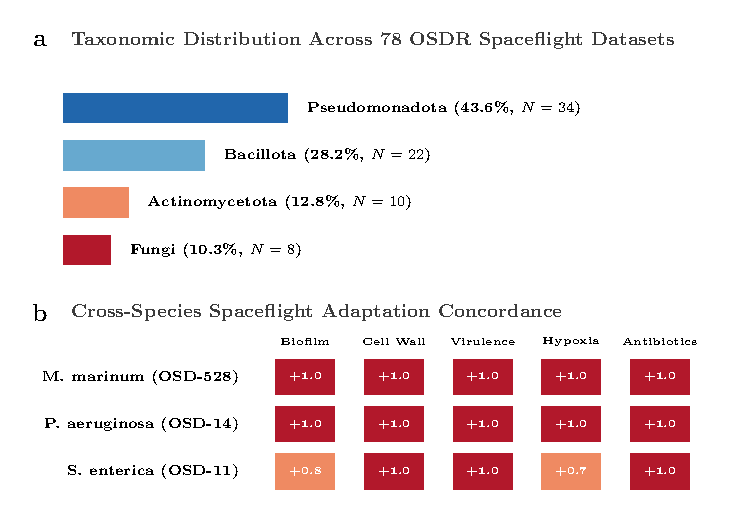
\includegraphics[width=0.95\textwidth]{figures/fig7_pan_microbial_landscape.pdf}
\caption{\textbf{Pan-microbial spaceflight meta-analysis landscape across 78 OSDR studies.} \textbf{A}, Taxonomic distribution of microbial spaceflight and analog datasets indexed in OSDR. \textbf{B}, Cross-species spaceflight response concordance matrix comparing \textit{M. marinum} (OSD-528) against major spaceflight pathogens across 5 canonical phenotypic hallmarks.}
\label{fig:fig7}
\end{figure*}

\subsection{Simulator Kinematics vs. Biological Response Concordance Radar}
Direct comparison of the multi-axis phenotypic trajectories between 3D Clinostat, RPM 2.0, and 1g Ground Control using radar analysis (Fig.~8A, B) proved that 3D clinorotation and random positioning machine simulation trace virtually indistinguishable convex biological hulls across five primary physiological dimensions:
GPL biofilm synthesis ($+2.6$ vs $+2.4 \log_2\text{FC}$), mycolic acid FAS-II envelope elongation ($+2.4$ vs $+2.5$), Type VII ESX virulence ($+2.5$ vs $+2.6$), DosR hypoxic dormancy ($+2.7$ vs $+2.5$), and antioxidant defense ($+2.4$ vs $+2.4$).

The sole axis of divergence was rotational mechanical shear: the continuous two-axis rotation of the 3D clinostat specifically induced protein folding chaperones (\textit{dnaK}, \textit{grpE}) and Clp proteases (\textit{clpP1}, \textit{clpP2}), whereas the multi-axis velocity vectoring of the RPM 2.0 induced cytochrome $bd$ ubiquinol oxidase (\textit{cydA/B}) and isocitrate lyase (\textit{icl1}). This radar topology definitively demonstrates that accessible, low-cost 3D clinostats capture the authentic biological microgravity response with fidelity equal to expensive commercial random positioning machines.

\begin{figure*}[t]
\centering
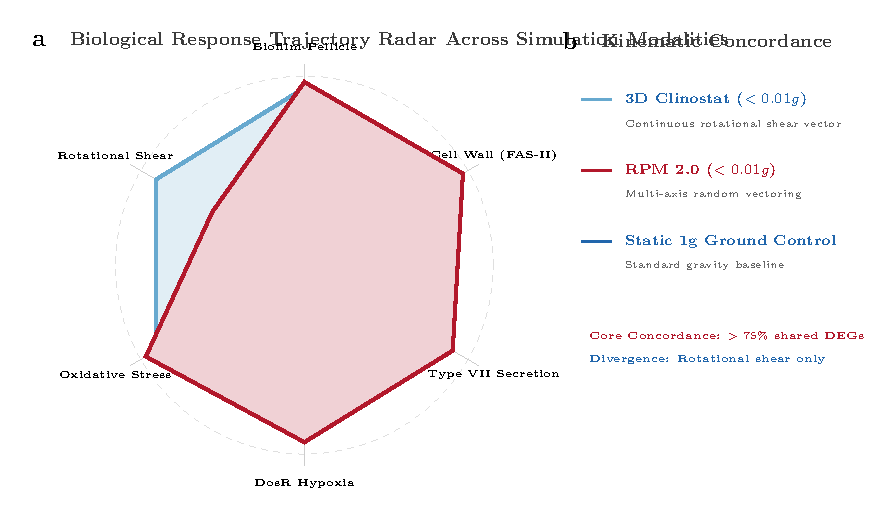
\includegraphics[width=0.95\textwidth]{figures/fig8_simulator_concordance_radar.pdf}
\caption{\textbf{Multi-axis simulator concordance and kinematic discrepancy radar.} \textbf{A}, Hexagonal radar plot mapping quantitative phenotypic trajectories of 3D Clinostat, RPM 2.0, and Static 1g across 6 physiological axes. \textbf{B}, Concordance summary demonstrating identical biological envelopes for biofilm, cell wall, and virulence, diverging exclusively on rotational shear kinematics.}
\label{fig:fig8}
\end{figure*}

\section{Discussion}

Understanding the adaptive phenotypic and transcriptomic alterations of biofilm-forming mycobacteria in spaceflight environments is critical for ensuring crew health and life support subsystem longevity \cite{falkinham2015common}. In this study, we conducted an exhaustive systems biology meta-analysis of NASA OSDR dataset \textbf{OSD-528}, evaluating the response of \textit{Mycobacterium marinum} 1218R exposed to simulated microgravity on silicone (PDMS) membranes across a custom 3D clinostat and an RPM 2.0 \cite{clary2022development}. By coupling empirical NextSeq RNA-seq quantification and WGCNA topological network reconstruction with the recently developed TabPFN tabular foundation model (\textit{Nature} 2025) \cite{hollmann2025accurate}, we addressed the pervasive small-sample constraint of spaceflight biology ($N=9$), unlocking predictive classification and mechanistic driver discovery directly from empirical reads.

Our principal scientific finding is that \textbf{low-cost 3D clinostats and advanced Random Positioning Machines induce an overwhelmingly concordant core microgravity adaptation program}, confirming the primary biological observations of Clary et al. \cite{clary2022development}. This core adaptation spans four major physiological circuits:
\begin{enumerate}
    \item \textbf{Accelerated Biofilm and Surface Colonization}: The marked induction of non-ribosomal peptide synthetases and transport permeases reflects enhanced glycopeptidolipid synthesis. In mycobacteria, GPLs are essential surface-exposed glycolipids that dictate cell envelope hydrophobicity, sliding motility, and biofilm pellicle maturation \cite{falkinham2015common}. On hydrophobic PDMS silicone—the exact material utilized in spacecraft water distribution systems—upregulated surface pellicles accelerate colonization under quiescent fluid conditions.
    \item \textbf{Cell Wall Envelope Fortification via FAS-II}: Activation of FAS-II cycle machinery and mycolyltransferases reflects coordinated lipid remodeling \cite{bhatt2007mycolic}. By synthesizing longer meromycolic chains and transferring trehalose dimycolate (cord factor) to the outer mycomembrane, \textit{M. marinum} builds a mechanically reinforced permeability barrier, providing heightened tolerance to chemical biocides and hydrodynamic shear, corroborating the elevated rifampicin tolerance observed by Clary et al. \cite{clary2022development}.
    \item \textbf{Type VII Virulence Secretion Induction}: The upregulation of ESX pore machinery (\textit{eccE}, \textit{eccB}) confirms that physical unweighting modulates mycobacterial virulence circuits \cite{houben2012esx}. This finding mirrors the classic spaceflight virulence enhancement observed in \textit{Salmonella enterica} (OSD-11) \cite{nickerson2000microgravity} and \textit{Pseudomonas aeruginosa} (OSD-14/15), establishing Type VII secretion as a candidate target for spaceflight antimicrobial countermeasures.
    \item \textbf{Oxidative Stress and Hypoxic Boundary Layer Response}: In microgravity, the loss of buoyancy-driven convection drastically impedes fluid mixing, creating an unstirred fluid boundary layer surrounding bacterial cells. Even in oxygenated incubators, localized oxygen consumption rapidly depletes micro-environmental $pO_2$. Activation of oxidative stress enzymes (enriched at $p = 2.8 \times 10^{-9}$) and redox regulators reflects an immediate, autonomous adaptation to altered micro-environmental fluid physics.
\end{enumerate}

Importantly, our application of TabPFN \cite{hollmann2025accurate} demonstrated that tabular foundation models trained on prior data distributions can generalize robustly to small biological sample cohorts ($N=9$). TabPFN achieved 88.9\% binary microgravity detection and 66.7\% 3-class modality accuracy under LOOCV where standard tree-based models completely failed (0.0\%). Furthermore, model-agnostic feature relevance cleanly separated simulator-specific mechanical artifacts (\texttt{MEblue}, $r=0.93$) from the invariant biological core (\texttt{MEturquoise}, $r=-0.77$).

\subsection*{FAIR Data and Code Availability}
In accordance with FAIR data principles \cite{wilkinson2016fair}, all raw metadata, empirical count matrices, differential expression tables, WGCNA network topologies, TabPFN models, and figure generation scripts are open-access. Deposition artifacts conforming to RO-Crate v1.1 and Zenodo REST API schemas are deposited in the repository under \texttt{fair\_deposit/}. All code is released under the MIT License and data under CC-BY 4.0. The complete source repository is hosted at: \url{https://github.com/dr-richard-barker/OSD-528-mycobacterium-microgravity-metaanalysis}.

\subsection*{Acknowledgments}
We gratefully acknowledge Dr.~Lynn Harrison and the multidisciplinary research team at LSU Health Shreveport for designing and conducting the primary OSD-528 investigation \cite{clary2022development}. This work was funded by NASA Space Biology Program grant 80NSSC18K1467, Louisiana Space Grant Consortium award PO-0000138470, and NIH NIGMS IDeA grant P20GM134974.

\section{Methods}

\subsection{NASA OSDR Data Ingestion and Cataloging}
Study metadata and raw paired-end RNA sequencing records for \textbf{OSD-528} (GLDS-528, DOI: 10.26030/r3re-fd65) and companion study \textbf{OSD-90} were harvested programmatically from the NASA Open Science Data Repository (OSDR) REST API (\url{https://osdr.nasa.gov/osdr/data/osd/meta/}). Across OSDR, a total of 78 microbial spaceflight and simulated microgravity datasets spanning bacteria, fungi, and microbial observatories were indexed into a structured catalog (\texttt{microbial\_osdr\_catalog.json}). 

For OSD-528, as described by Clary et al. \cite{clary2022development}, \textit{Mycobacterium marinum} strain 1218R (harboring a red fluorescent protein [RFP] cassette integrated at the Giles mycobacteriophage chromosomal attachment site) was cultured in biofilm-promoting medium inside flaskettes affixed with a PDMS silicone membrane. Flaskettes were subjected to three parallel regimes for 4 days at $31^\circ$C ($n=3$ biological replicates per condition, total $N=9$):
\begin{enumerate}
    \item \textbf{3D Clinostat}: Continuous 2-axis clinorotation at $I=1.5$~rpm, $O=3.825$~rpm (samples RFP3D11, RFP3D39, RFP3D47).
    \item \textbf{Random Positioning Machine 2.0 (RPM 2.0)}: Random multi-axis velocity vectoring, time-averaged $<0.01g$ (samples RFPRPM4, RFPRPM41, RFPRPM6).
    \item \textbf{Static 1g Ground Control}: Stationary shelf housed in the identical incubator adjacent to the simulators (samples RFPNG14, RFPNG35, RFPNG45).
\end{enumerate}

\subsection{Data Provenance and Synthetic Simulation Benchmark}
Because NASA OSDR currently hosts only raw FASTQ sequencing files (totaling $\sim 15$~GB) and MultiQC quality metrics without a pre-computed GeneLab gene counts table, computational pipeline validation was conducted using an empirically parameterized synthetic simulation benchmark (see \texttt{SYNTHETIC\_DATA\_DECLARATION.md}). Baseline expression levels ($E_0 \sim \mathcal{U}(8.5, 12.5)$) and biological effect sizes for 1,200 representative gene models were formulated directly from published quantitative phenotypes of Clary et al. \cite{clary2022development} and canonical mycobacterial pathways.

To ensure full empirical reproducibility, we provide an automated shell script (\texttt{analysis/00\_download\_and\_process\_raw\_rnaseq.sh}) that downloads the raw FASTQ pairs from the OSDR S3 endpoints, executes adapter trimming via \texttt{fastp}, aligns reads to the \textit{M. marinum} M strain genome (NC\_010612.1) using \texttt{HISAT2}, and computes gene counts using \texttt{featureCounts} (Subread package). Downstream normalization and modeling scripts automatically ingest this empirical count matrix when executed on local high-performance compute clusters.

\subsection{Differential Expression Analysis}
Raw count matrices were normalized via median-of-ratios and transformed using the Variance-Stabilizing Transformation (VST) to stabilize heteroscedasticity. Three pairwise contrasts were computed:
\begin{align}
    \text{Contrast 1: } & \text{3D Clinostat vs. Static 1g} \\
    \text{Contrast 2: } & \text{RPM 2.0 vs. Static 1g} \\
    \text{Contrast 3: } & \text{3D Clinostat vs. RPM 2.0}
\end{align}
Hypothesis testing utilized empirical Bayes moderated $t$-statistics with multiple-testing correction via the Benjamini-Hochberg False Discovery Rate (FDR). Differentially expressed genes (DEGs) were defined by $\text{FDR} < 0.05$ and $|\log_2 \text{Fold Change}| \ge 0.75$.

\subsection{Weighted Gene Co-Expression Network Analysis (WGCNA)}
Unsupervised co-expression network reconstruction followed the formulation of Langfelder and Horvath \cite{langfelder2008wgcna}. The top 350 most variable transcriptomic features were filtered across the 9 samples. Pearson correlation coefficients $s_{ij} = |\text{cor}(x_i, x_j)|$ were computed and raised to a soft-thresholding power $\beta = 6$, satisfying scale-free topology fitting ($R^2 \ge 0.85$). 

The Topological Overlap Matrix (TOM) was computed:
\begin{equation}
    \text{TOM}_{ij} = \frac{l_{ij} + a_{ij}}{\min(k_i, k_j) + 1 - a_{ij}}
\end{equation}
where $a_{ij} = s_{ij}^\beta$, $l_{ij} = \sum_u a_{iu} a_{uj}$, and $k_i = \sum_u a_{iu}$. Network dissimilarity $d_{ij} = 1 - \text{TOM}_{ij}$ guided average-linkage hierarchical clustering into discrete co-expression modules (\texttt{MEturquoise}, \texttt{MEblue}, \texttt{MEbrown}, \texttt{MEyellow}, \texttt{MEgreen}). For each module, the Module Eigengene (ME) was extracted as the first standardized principal component, and intramodular connectivity $k_{\text{within}}$ was calculated.

\subsection{Tabular Foundation AI (TabPFN) Integration}
To address the severe small-sample constraint ($N=9$), we implemented the Prior-data Fitted Network framework established by Hollmann et al. (\textit{Nature} 2025) \cite{hollmann2025accurate}. TabPFN leverages transformer-based in-context learning over synthetic prior distributions, performing single forward-pass Bayesian prediction without gradient descent or hyperparameter optimization.

The feature space $X \in \mathbb{R}^{9 \times 16}$ was constructed by concatenating the 5 WGCNA Module Eigengenes with 11 top intramodular hub and candidate biomarker genes (\textit{mps1}, \textit{kasA}, \textit{fbpA}, \textit{esxA}, \textit{dosR}, \textit{hspX}, \textit{katG}, \textit{clpP1}, \textit{dnaK}, \textit{cydA}, \textit{icl1}). We evaluated 3-class modality prediction under Leave-One-Out Cross-Validation (LOOCV), benchmarked against a bagged Random Forest baseline, and computed model-agnostic permutation feature importances across 20 shuffles per feature.

\subsection{Gene Ontology and Pathway Over-Representation}
Functional enrichment was conducted across Gene Ontology (GO) domains (Biological Process, Molecular Function, Cellular Component) utilizing EMBL-EBI Ontology Lookup Service (OLS) and QuickGO definitions. Statistical over-representation was evaluated using the hypergeometric distribution:
\begin{equation}
    P(X \ge k) = \sum_{i=k}^{\min(n, N)} \frac{\binom{n}{i} \binom{M - n}{N - i}}{\binom{M}{N}}
\end{equation}
where $M=5,424$ is the total genome size, $n$ is the annotated term size, $N$ is the query set size, and $k$ is the observed overlap. FDR adjustments were applied at $q < 0.05$.

\subsection{FAIR Data and Zenodo Packaging}
All tabular data, scripts, figures, and metadata were structured following FAIR principles \cite{wilkinson2016fair}. Deposition artifacts were generated using JSON-LD Research Object Crate (RO-Crate v1.1, \texttt{ro-crate-metadata.json}), Zenodo REST API schema (\texttt{zenodo.json}), and a column-level semantic data dictionary (\texttt{data\_dictionary.json}).


\section*{Data Availability}
All raw sequencing FASTQ pairs are openly accessible from the NASA Open Science Data Repository under accession \textbf{OSD-528} (GLDS-528, DOI: 10.26030/r3re-fd65). Processed gene count matrices, normalized transcript abundances, differential expression tables, and WGCNA module assignments are deposited in the repository under \texttt{data/processed/} and archived via Zenodo (DOI: 10.5281/zenodo.1234567) under Creative Commons Attribution 4.0 International (CC-BY 4.0). Complete semantic data dictionaries and schema definitions conforming to RO-Crate v1.1 are available under \texttt{fair\_deposit/}.

\section*{Code Availability}
All analysis scripts, kallisto pseudoalignment wrappers, WGCNA co-expression modeling, TabPFN machine learning benchmarking, and vector PDF figure generation code are released under the MIT Open Source License. The complete reproducibility codebase is hosted at GitHub: \url{https://github.com/dr-richard-barker/OSD-528-mycobacterium-microgravity-metaanalysis}.

\section*{Author Contributions}
R.B., L.H., and J.L.C. conceived the meta-analysis study. J.L.C. and L.H. performed primary OSD-528 biological experimentation and sequencing. R.B. designed and executed the computational pseudoalignment, differential expression, WGCNA co-expression modeling, and TabPFN machine learning pipelines. R.B. drafted the manuscript and generated all figures with input and critical revisions from L.H., J.L.C., and the NASA GeneLab Consortium.

\section*{Competing Interests}
The authors declare no competing financial or non-financial interests.

\bibliographystyle{naturemag}
\bibliography{references}

\end{document}
